\section{Autosub Submission System} \label{autosub_system}

The autosub submission system has the following responsibilities:
\begin{itemize}
    \item Fetch, process, send and archive student E-Mails.
    \item Store and manage tasks, users and submissions.
    \item Initiate generation of tasks and testing of submissions.
    \item Produce statistics.
\end{itemize}

In the following {\it Structured Analysis} will be used to specify the
system. If you are not familiar with this method, you can find details e.g. in
\cite{demarco, gooma, cooling}.

\begin{figure}[h!]
    \begin{center}
    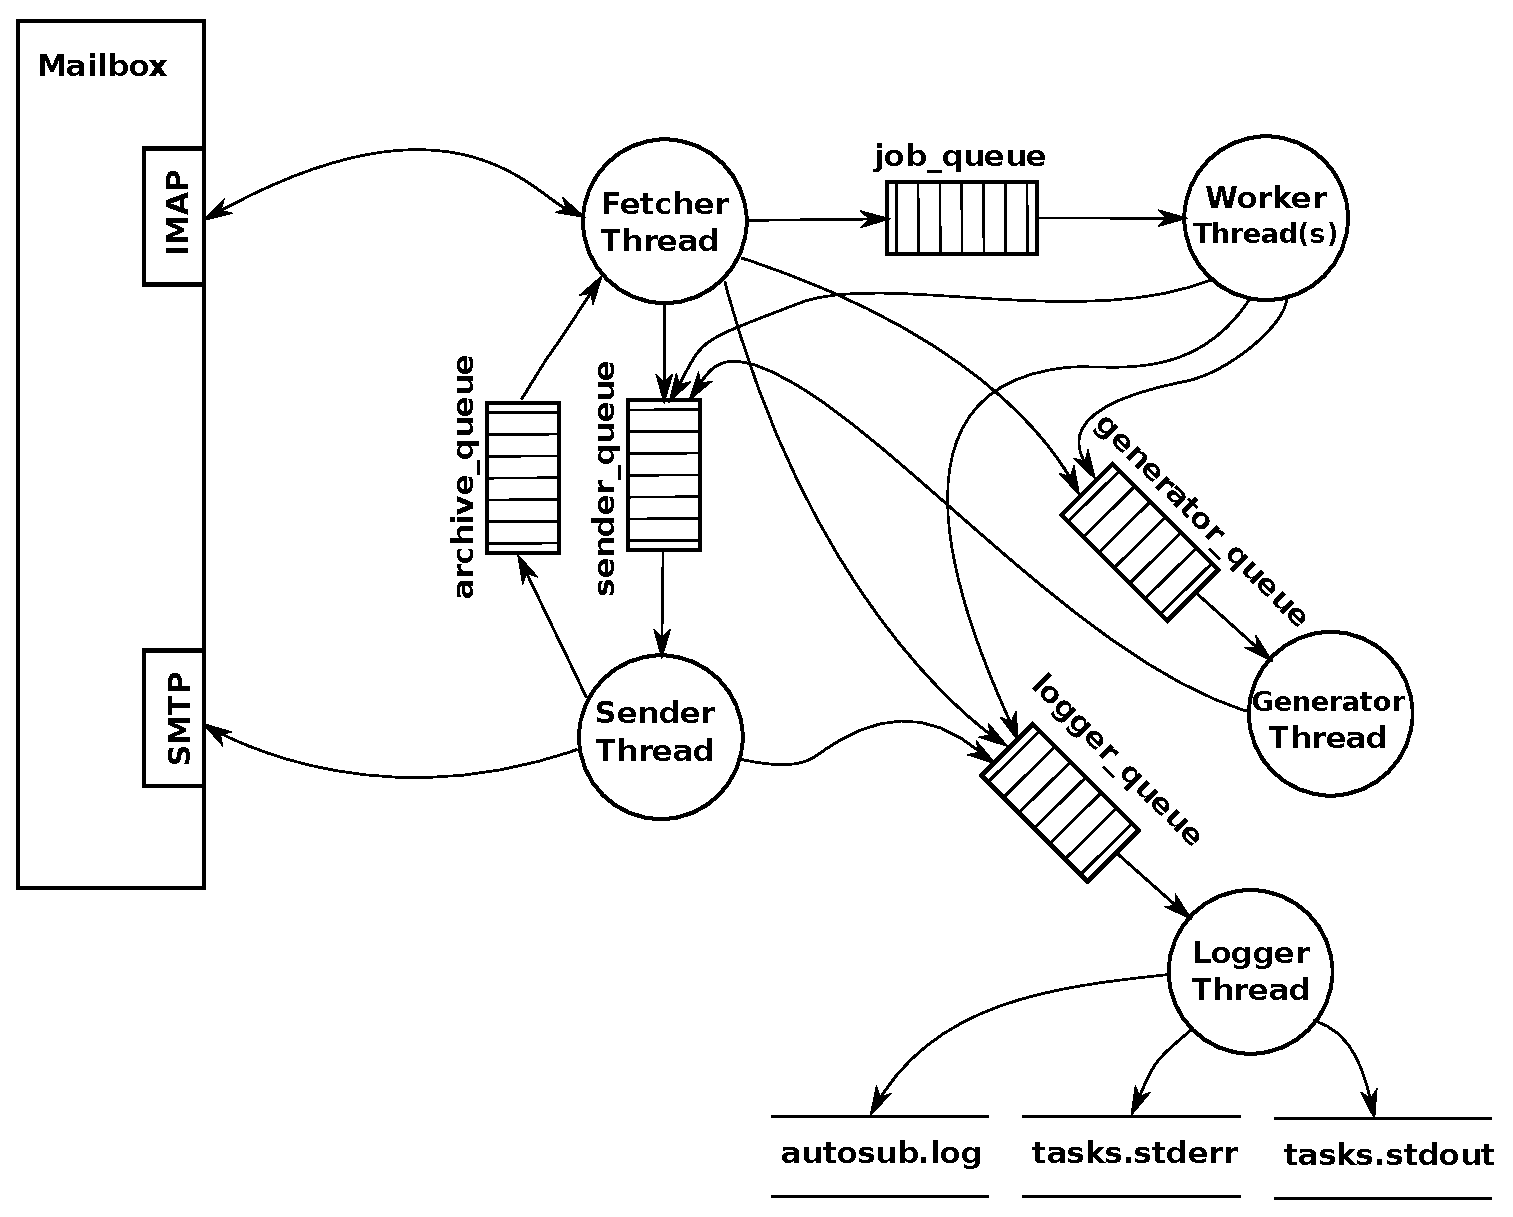
\includegraphics[width=11cm]{images/autosub_structure.eps}
    \caption{DFD0 -- High-Level Data-Flows in the Submission System.}
    \label{fig:dfd0}
    \end{center}
\end{figure}

The autosub submission system is a daemon implemented in Python3 that is 
composed of multiple threads communicating over queues. This multi-threading 
approach is especially important for the testing process. As the test of a single
task can take rather long and each student can hand in (correct and incorrect) 
solutions. Furthermore the goal is to assure, that there still is progress, even 
if a test is running. A view of the parts and data-flows of the autosub system can 
be seen in Figure \ref{fig:dfd0}. The individual entities are described in the next subsection,
the message queues in the Appendix Section \ref{app:queues}.

\subsection{Description of Entities} \label{autosub_entities}
\begin{description}
    \item [MB] \textbf{Mailbox} \\
    \begin{tabular}{|p{2cm}|p{11cm}|}
        \hline
        Description & Mailbox to interface with students. \\
        \hline
        Rate & Asynchronously by students, periodically with configurable interval by
		the E-Learning system. \\
        \hline

        Comment & The Mailbox is used to interface with the students.
        The Mailbox is accessed via \gls{imap} for reading new E-Mails and \gls{smtp} 
		to send E-Mails.

        After the action triggered by an received E-Mail has been processed, the E-Mail 
		is archived into a configurable folder on the \gls{imap} server.
        \\
        \hline
    \end{tabular}
    \item [1] \textbf{Fetcher thread} \\
    \begin{tabular}{|p{2cm}|p{11cm}|}
        \hline
        Description &  Fetch E-Mails from the Mailbox.\\
        \hline
        Rate & Periodically with configurable interval. \\
        \hline
        Comment & The Fetcher thread periodically checks the Mailbox for new E-Mails. 
		This thread initiates actions based on the user E-mail address and the subject.
		Further information concerning the E-Mail interface can be be seen in Section 
		\ref{emailinterface} 
        \\
        \hline
    \end{tabular}

	\item [2] \textbf{Generator thread} \\
    \begin{tabular}{|p{2cm}|p{11cm}|}
        \hline
        Description & Generate a (unique) example for a user. \\
        \hline
        Rate & Asynchronously triggered  by the E-Learning System when a new task for a user has 
		to be created.\\
        \hline
        Comment & The Generator thread initiates generation of unique tasks for students.
  		The Generator thread is blocking on the generator\_queue, until the generation 
		of a new example is requested. As soon as the example was generated, a request 
		to send it out is put into the sender\_queue.
        \\
        \hline
    \end{tabular}
   
	\item [3] \textbf{Worker thread(s)} \\
    \begin{tabular}{|p{2cm}|p{11cm}|}
        \hline
        Description & Test the task submissions of students. \\
        \hline
        Rate & Asynchronously triggered upon arrival of a new task submission 
		by a student. \\
        \hline
        Comment & The Worker threads are the ones which do the initiate testing 
		submissions by a student. If the Fetcher thread receives an E-Mail with a result 
		submission, a new message is added to the job\_queue. The worker threads are 
		using a blocking read on the job\_queue to wait for work, as soon as the new 
		message is added by the Fetcher thread one of the workers will read it and 
		start the tests for the users submission.
        \\
        \hline
    \end{tabular}

    
	\item [4] \textbf{Logger thread}\label{sec:logger} \\
    \begin{tabular}{|p{2cm}|p{11cm}|}
        \hline
        Description & Format log messages and store them in the log file. \\
        \hline
        Rate & Asynchronously triggered by all other threads. \\
        \hline
		Comment & In order to enforce a common logging format, and allow the setting 
		of a common log-level, all threads just put their log-messages into the 
		logger\_queue. The Logger thread decides (depending on the log-level and configured 
		log-threshhold) whether or not the message shall be logged or not. If so, the message
		is formatted and written to the log file. The log-level threshold can be configured in the
		config file.

		The following log-levels are implemented (from lowest to highest):
        \begin{description}
		\item [DEBUG:] Print all kind of information that might be helpful to debug
			problems. This includes, what user sent which E-Mail, what action
			was taken, what was the result of that action.
		\item [INFO:] Information that might be of interest, even if not in debugging
			mode.
		\item [WARNING:] A problem occurred, but it did not lead to a long-term problem
			(e.g. could not connect to the mailserver, but after retrying it worked).
		\item [ERROR:] A problem that lead to a long-term malfunction of the submission
			system occurred, the system will not be able to recover from this problem.
		\end{description}
        \\
        \hline
    \end{tabular}

	\item [5] \textbf{Sender thread} \\
    \begin{tabular}{|p{2cm}|p{11cm}|}
        \hline
        Description & Sends E-Mails to the students \\
        \hline
        Rate & Asynchronously by Fetcher, Worker or Generator thread. \\
		\hline
		Comment & If a message has to be returned to the student, the thread that 
		wants to send the message just puts the necessary information into the 
		sender\_queue. The sender thread then takes that information, formats an 
		E-Mail and sends it out using \gls{smtp}.

        The unique message-id is passed from the fetcher (possibly via other 
		threads) to the sender thread. If the sender thread has sent out the 
		answering E-Mails, the E-Mail with the given message-id is moved into an 
		archive folder on the mail server.
        \\
        \hline
    \end{tabular}

	\newpage 

	\item [6] \textbf{Dailystats thread} \\
    \begin{tabular}{|p{2cm}|p{11cm}|}
        \hline
        Description & Creates statistical information. \\
        \hline
        Rate & Activated every 12 hours. \\
		\hline
		Comment & The dailystats thread is used to get a timeline of some very basic statistics.
		Currently the number users, sent E-Mails, received E-Mails and received questions
		over time are evaluated and plotted into a graph. The graphs are stored and 
		can e.g. be viewed in the Statistics tab of the VELS web interface.
        \\
        \hline

    \end{tabular}
\end{description}

\subsection{Datastores}
For storing data two databases are used. The name and location of those databases 
can be configured through the configuration file, in the following we will refer to 
them with the default name that is used, if no other name is provided in the 
configuration file:
\begin{description}
\item [semester.db: ] The {\tt semester.db} database is used to store all data that is
    specific to one semester. This includes, users, parameterization of tasks assigned
    for users, statistics, etc. The {\tt semester.db} default location is in
	{\tt "autosub/src"}.
\item [course.db: ] The {\tt course.db} database consists of configuration data that will
    very likely be reused in multiple semesters. This separation makes it very easy
    to start a new semester: just backup {\tt semester.db} to some safe location and
    remove it in the original location (a new empty one will be made automatically upon 
    starting the autosub daemon). Then use the VELS web interface to perform the small 
    modifcations(year/semester,deadlines, etc.) needed in {\tt course.db}. The
    {\tt course.db} default location is in {\tt "autosub/src"}.
\end{description}
Specifics about the tables of these databases can be found in the Appendix Section
\ref{app:semester.db} and \ref{app:course.db}.

In addition there is one important directory that is used by autosub to store data in,
the directory: {\tt autosub/src/users}. In this directory a unique directory for every
user is created, and this directory the description of each individual received task 
and submissions for the individual tasks are stored. Every directory has the form 
{\tt "autosub/src/users/<user\_id>/Task<nr>/"}. Submissions are stored in separate 
folders which are named {\tt "Submission<nr>\_<date>\_<time>/"}. Task description files 
are stored in the folder named {\tt "desc/"}.

\subsection{Config File}
The autosub system uses a config file (.cfg) which is passed to the daemon to configure the
individual threads and overall system. The file is read when starting the daemon. If no
.cfg file is specified, the used file is default.cfg located in {\tt "autosub/src/"}. 
Information about the config file can be found in the Appendix Section \ref{app:config}
and an example config file in in Section \ref{sub:exampleconfig}.

\subsection{Logging and error detection} \label{logerror}

The autosub system is implemented as a daemon process. As such it does not
directly print any information to the {\tt stdout} (i.e. the screen), instead
all messages for the administrator are stored in log files. All log and error files
are stored in a configurable directory (default {\tt "autosub/src"}).

\begin{description}
\item [autosub.log] This is the main log file that is used by the actual autosub
daemon software to log everything. The format in this log file is as follows:

\begin{verbatim}
<date> <time> [<logger name>] <loglevel> <logmessage>
\end{verbatim}

Here is a small section of {\tt autosub.log} taken from startup -- first the daemon checks
whether a directory {\tt users} used to store the users submissions is existing, then
it checks if necessary tables in the database exist. After those checks have been
done further threads (described in Section \ref{autosub_entities}) are started, and
announce themselves.

{\scriptsize
\begin{verbatim}
2015-09-17 22:23:40,629 [autosub.py  ] WARNING: Directory already exists: users
2015-09-17 22:23:40,630 [autosub.py  ] DEBUG: table SpecialMessages does not exist
2015-09-17 22:23:43,679 [autosub.py  ] DEBUG: table TaskConfiguration does not exist
2015-09-17 22:23:43,955 [autosub.py  ] DEBUG: table GeneralConfig does not exist
2015-09-17 22:23:45,878 [sender      ] INFO: Starting Mail Sender Thread!
2015-09-17 22:23:45,884 [fetcher     ] INFO: Starting Mail Fetcher Thread!
2015-09-17 22:23:45,884 [fetcher     ] DEBUG: Imapserver: 'mail.intern.tuwien.ac.at'
2015-09-17 22:23:45,884 [generator   ] INFO: Task Generator thread started
2015-09-17 22:23:45,890 [activator   ] INFO: Starting activator
2015-09-17 22:23:45,890 [Main        ] INFO: Used config-file: testzid.cfg
2015-09-17 22:23:45,891 [Worker1     ] INFO: Starting Worker1
2015-09-17 22:23:45,892 [Main        ] INFO: All threads started successfully
2015-09-17 22:23:45,892 [Worker1     ] INFO: Worker1: waiting for a new job.
2015-09-17 22:23:45,893 [Worker2     ] INFO: Starting Worker2
\end{verbatim}
}

As you can see from theses examples, a lot of information is available, with
exact timestamps and a way to know which thread the message is coming from.
In addition the debug level gives a sense of how important (or even critical)
the message is. The log-level threshhold can be configured using the config file.

\end{description}

Autosub tries to give information on severe problems on all available channels. An example would be,
if no task is configured, the email sent to the student will contain the message that
something went wrong as well -- although the error can be seen in the {\tt autosub.log}
file as well.

